\section{Derivations}
\label{sec:appendix-proofs}

\paragraph{Identities.} Conditioning on the verifier outcome,
$P(Y^\ast=1)=P(Y^\ast=1\mid\hat Y=1)P(\hat Y=1)+P(Y^\ast=1\mid\hat Y=0)P(\hat Y=0)
=a(1-q)+(1-a)r$; conditioning on the joint cell gives Eq.~\eqref{eq:joint}.
Bayes' rule gives $\alpha=aq/(1-A^\ast)$ and $\beta=(1-a)r/A^\ast$;
substituting these into $(a-\alpha)/(1-\alpha-\beta)$ recovers $A^\ast$
exactly (checked symbolically in the released code), substituting $q,r$
directly does not.

\paragraph{Sharpness.} $\Delta^\ast=\sum_j k_j\theta_j+\text{const}$ with
coefficients $k_j$ given by census shares ($s_{1c}-s_{2c}$ for a pooled
parameter; $s_{1c}$ and $-s_{2c}$ for model-specific ones). Over a box
$\prod_j[\theta_j^-,\theta_j^+]$ the minimum takes $\theta_j^-$ where
$k_j>0$ and $\theta_j^+$ where $k_j<0$, the maximum the reverse; both are
attained, so the range is sharp.

\paragraph{Pooling one verifier's rates.} With common $(q,r)$,
$\Delta^\ast=(a_1-a_2)(1-q-r)$, whose sign is that of $a_1-a_2$ whenever
$q+r<1$.

\section{Coverage}
\label{sec:appendix-coverage}

Fix an ordering $(1,2)$. Let $E_{\text{aud}}$ be the event that every
estimated parameter it depends on lies in its Clopper--Pearson interval, and
$E_{\text{samp}}$ the event that the benchmark-sampling interval for the
accuracy difference covers its target. The $k$ estimated parameters are
proportions from disjoint audited samples (different cells, or different
models' items), so with per-parameter level $0.975^{1/k}$,
$P(E_{\text{aud}})\ge0.975$ (Clopper--Pearson intervals are conservative, so
the bound holds exactly, not asymptotically). $P(E_{\text{samp}})\approx0.975$
from the normal approximation for a difference of two proportions over
1{,}324 items. On $E_{\text{aud}}$, $\Delta^\ast$ lies in the projected range
(sharpness above); on $E_{\text{aud}}\cap E_{\text{samp}}$, the widened
interval covers the superpopulation difference. By the union bound
$P(E_{\text{aud}}\cap E_{\text{samp}})\ge1-0.025-0.025=0.95$, with no
independence assumption between the audit sample and the benchmark items.
Parameters bounded logically ($[0,1]$ for unaudited disagreement cells, or
the stated bound under bounded heterogeneity) are not estimated and use no
coverage. Under homogeneity the audit part depends only on the two pooled
parameters and so holds for all orderings at once; the simultaneous variant
reported in Section~\ref{sec:results-joint} additionally puts the sampling
part at $0.025/136$ per ordering. The coverage is conditional on the stated
assumption (homogeneity or bounded heterogeneity); it does not account for
the assumption being false.

\section{Why full disagreement auditing stops short of the ceiling}
\label{sec:appendix-census}

If every disagreement response were audited and each model's disagreement
rates equalled the pooled audited value, \nCensusComb{} of the \nCeiling{}
sampling-permitted orderings would be resolved. \nCensusGapShrink{}
sampling-permitted orderings fail, and one ordering that sampling alone does
not resolve becomes resolved. The failures are not for lack of audit
information: correcting the disagreement mass shrinks the accuracy gap below
sampling error, so the pair's \code{score\_boxed} gap is significant but its
corrected gap is not (\nCensusGapShrinkCmdr{} of them involve \code{command-r-v01},
whose \code{score\_boxed} accuracy is mostly disagreement mass). This
projection fixes the disagreement rates at the pooled value and is
illustrative only.

\section{Simulation: plug-in versus two-phase estimator}
\label{sec:appendix-sim}

Finite benchmark of $N=1{,}324$ items; verifier errors drawn with the stated
$(\alpha,\beta)$; audit by simple random sampling within verifier strata
(6--40 items per stratum); 4{,}000 replicates. ``Plug-in'' feeds the audited
stratum rates into $(a-\alpha)/(1-\alpha-\beta)$. Coverage is for the
\v{S}id\'ak-adjusted Wilson projection used in this check.

\begin{center}\small
\resizebox{\linewidth}{!}{\begin{tabular}{@{}lccccc@{}}
\toprule
Scenario ($A^\ast,\alpha,\beta$) & bias, Eq.~(\ref{eq:identity}) & bias, plug-in & cover, Eq.~(\ref{eq:identity}) & cover, plug-in & empty, plug-in \\
\midrule
typical (0.2, 0.01, 0.02) & -0.0001 & -0.027 & 1.000 & 0.998 & 0.00 \\
low accuracy (0.02, 0.01, 0.02) & +0.0002 & -0.560 & 1.000 & 0.237 & 0.60 \\
zero accuracy (0.0, 0.01, 0.0) & +0.0000 & --- & 1.000 & --- & 1.00 \\
high error (0.4, 0.1, 0.15) & -0.0003 & -0.078 & 1.000 & 0.961 & 0.00 \\
perfect verifier (0.2, 0.0, 0.0) & +0.0000 & +0.000 & 1.000 & 1.000 & 0.00 \\
\bottomrule
\end{tabular}
}
\end{center}

\section{One-verifier audit design}
\label{sec:appendix-single}

\begin{figure}[h]
  \centering
  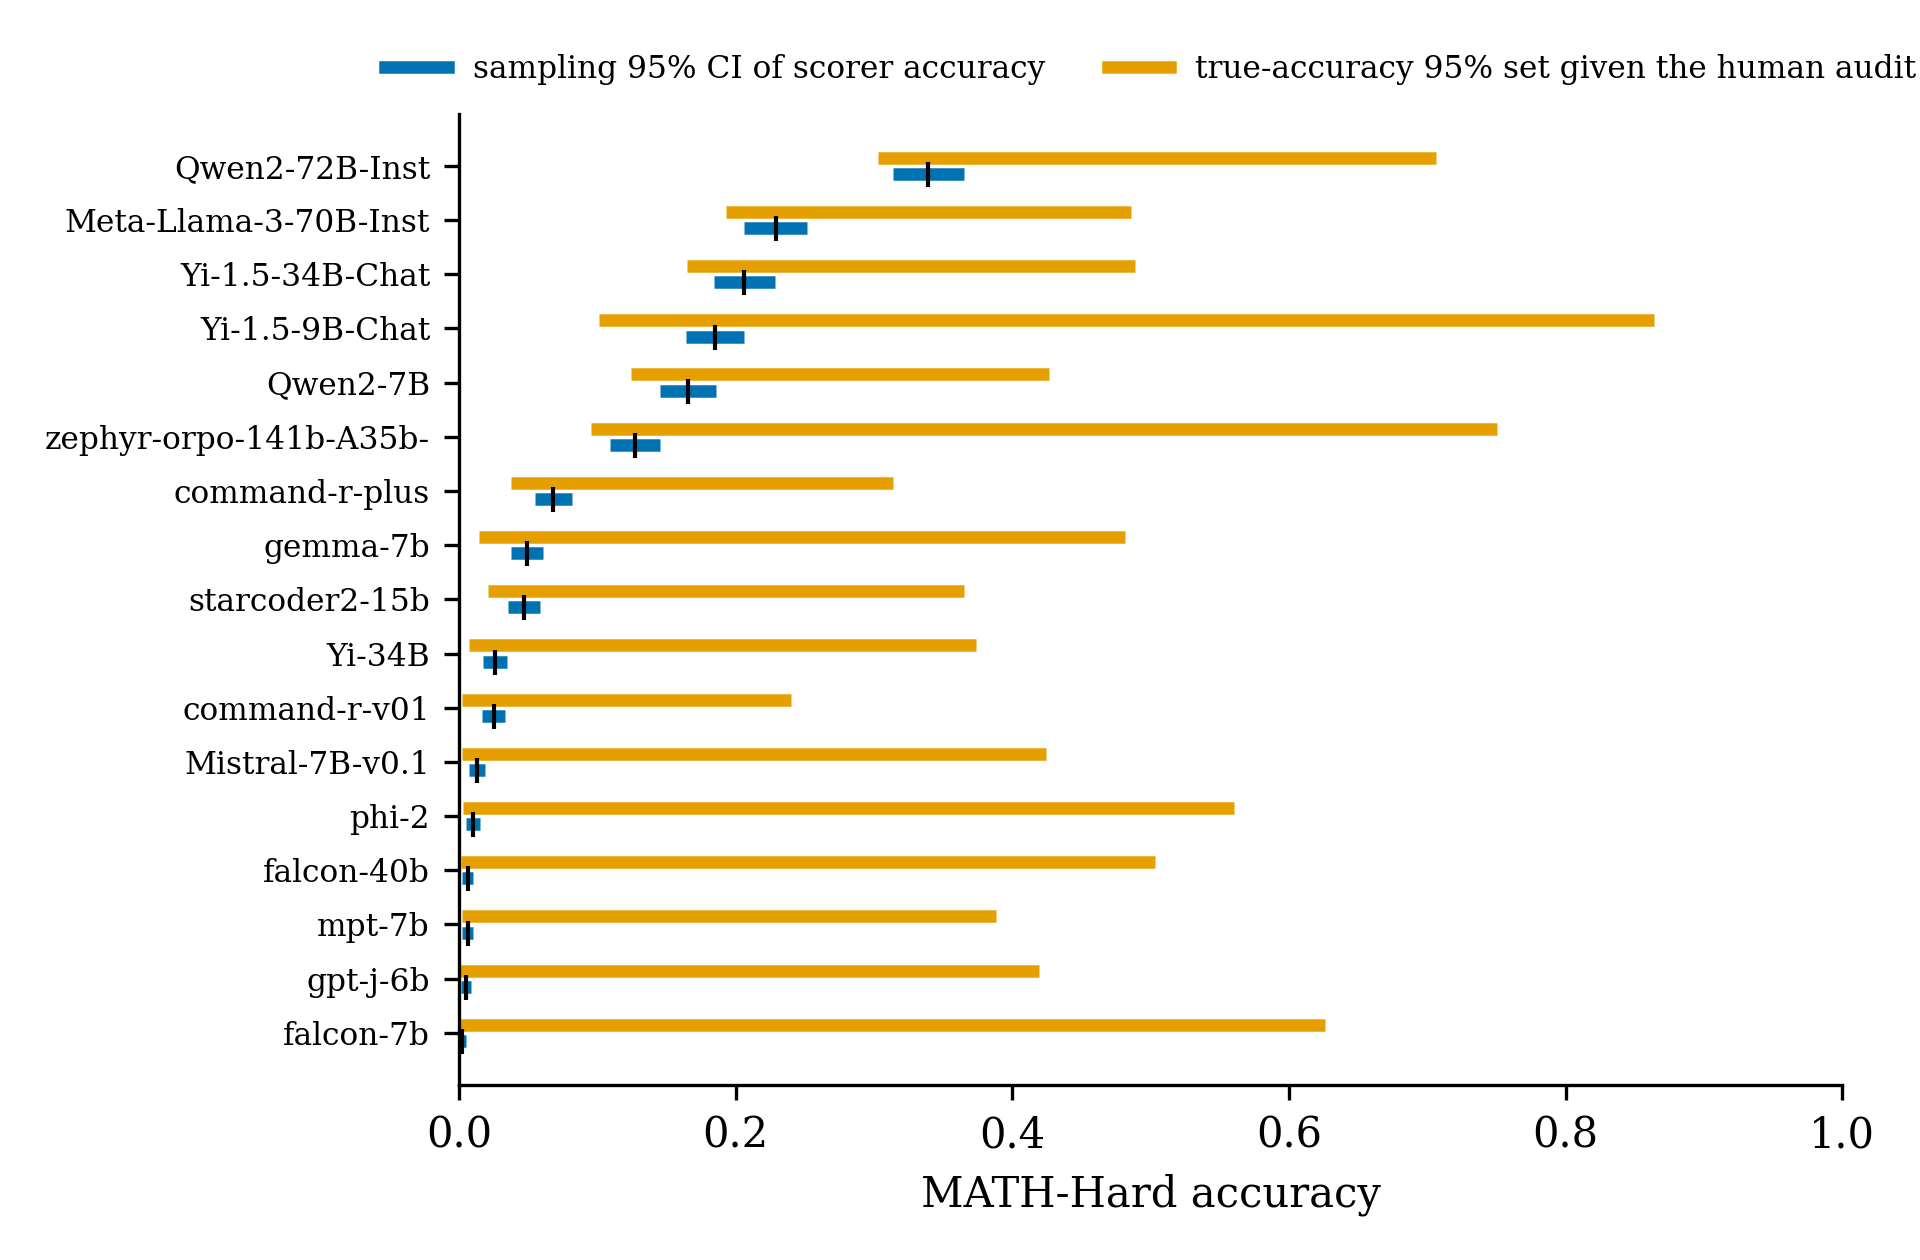
\includegraphics[width=0.50\linewidth]{figA_per_model_intervals.png}
  \caption{Per-model \code{score\_boxed} accuracy: sampling 95\% CI (blue)
  and true-accuracy set from the one-verifier, per-model audit (orange;
  Eq.~\eqref{eq:identity}, \v{S}id\'ak-adjusted Wilson intervals; illustrative).}
  \label{fig:intervals}
\end{figure}

\begin{figure}[h]
  \centering
  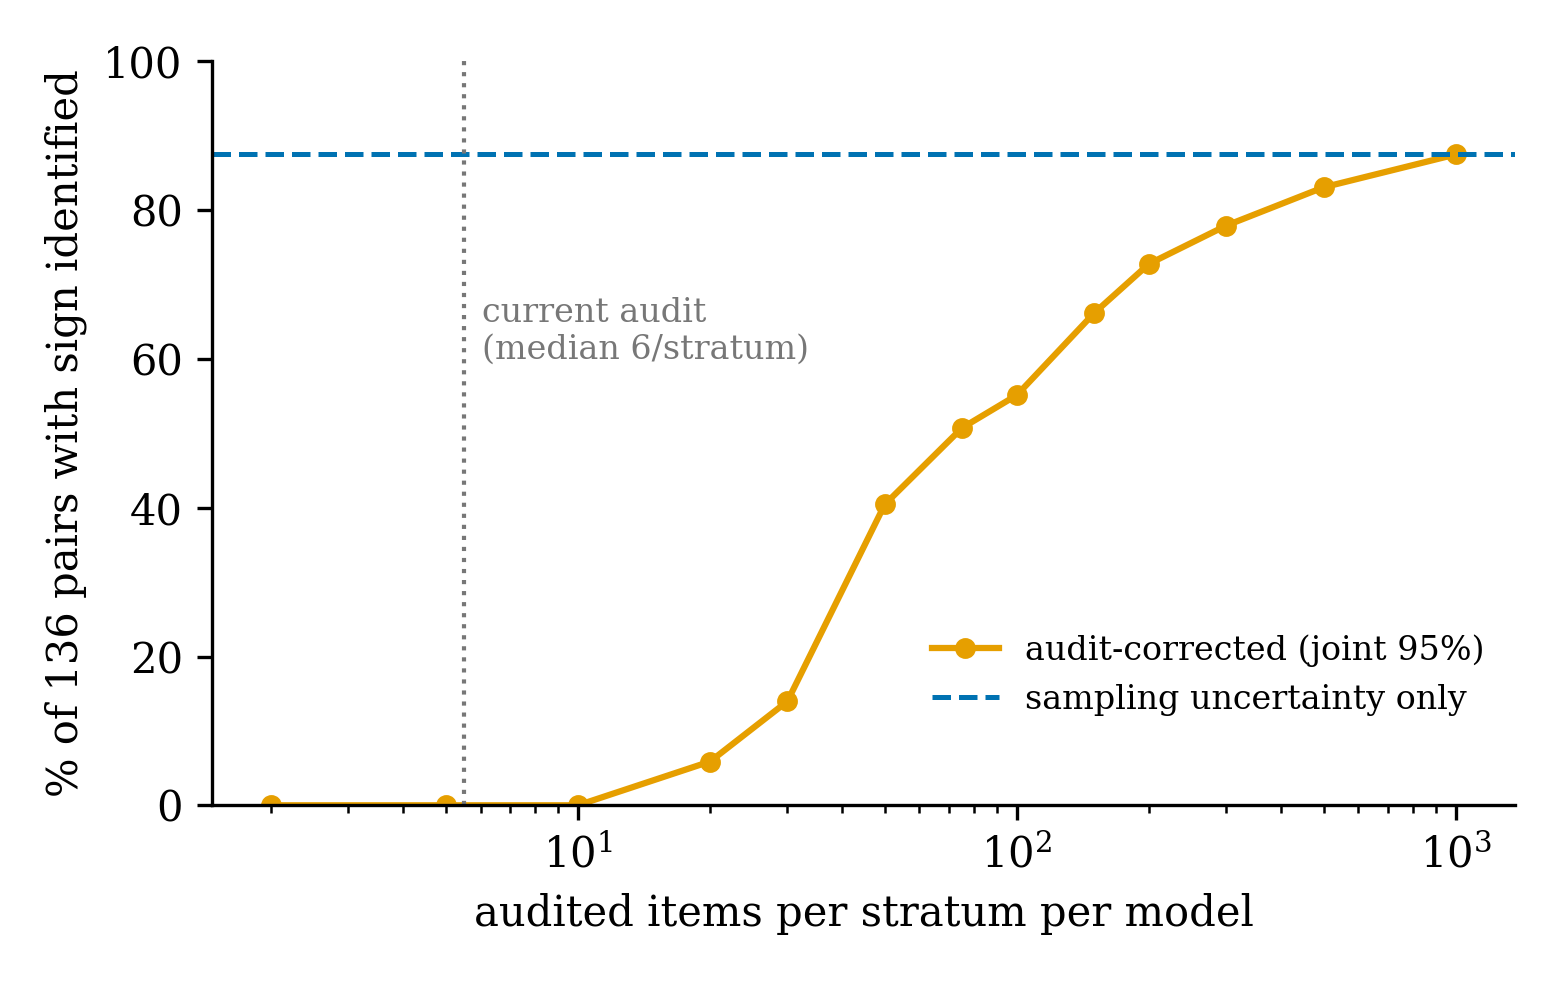
\includegraphics[width=0.44\linewidth]{figB_audit_sizing.png}
  \caption{One verifier, per model (audit only, Wilson): share of orderings
  resolved as audited items per stratum per model grow, each model's
  observed error rates held fixed.}
  \label{fig:sizing}
\end{figure}

For a model with zero observed errors in $n$ items per stratum the Wilson
width is about $z^2/(n+z^2)$; equating it with the sampling width
$2z\sqrt{a(1-a)/N}$ gives $n^\ast\approx(z/2)\sqrt{N/(a(1-a))}-z^2$, i.e.
\nNstarLow, \nNstarMid{} and \nNstarHigh{} items per stratum per model at
$a=0.35,0.20,0.05$. Simulated fresh audits (200 replicates, four truth
scenarios, \nCurTotal{} determinate labels scaled by 1--64) compare five
allocation rules at equal budget; plug-in Neyman resolves nothing at any
budget, and the rule minimizing summed zero-event widths
($n\propto\sqrt{a_m}$, $\sqrt{1-a_m}$) is best or tied. Curves:
\code{reaudit\_results.json}.

\section{Common-mechanism diagnostic}
\label{sec:appendix-mechanism}

\begin{figure}[h]
  \centering
  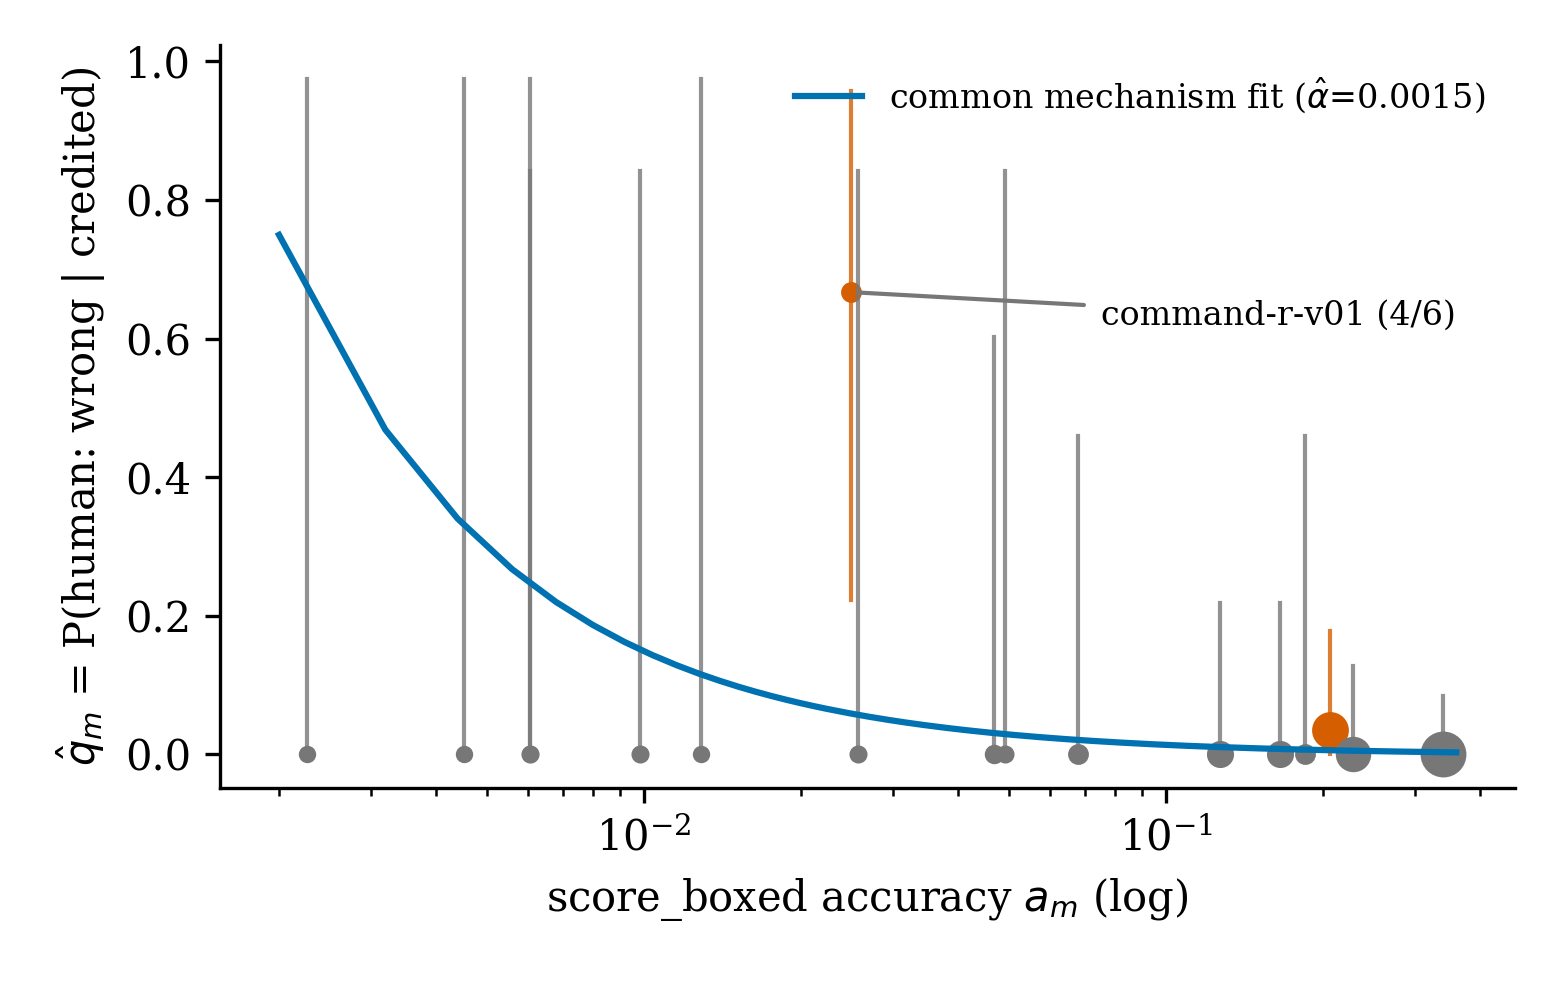
\includegraphics[width=0.44\linewidth]{figC_differential_error.png}
  \caption{Observed $\hat q_m$ (exact 95\% CI) against \code{score\_boxed}
  accuracy, with the rate implied by one common error mechanism.}
  \label{fig:differential}
\end{figure}

Under one $(\alpha,\beta)$ for all models, each model's $(q_m,r_m)$ is
implied by $a_m$. The grid maximum-likelihood fit gives
$\hat\alpha=\nAlphaHat$, $\hat\beta=0$, and a likelihood ratio of \nLR{}
against per-model rates (parametric bootstrap $p=\nLRp$).
\code{command-r-v01} contributes \nCmdrLR{}; leaving it out gives $p=\nLOOCmdrP$,
leaving out any other model gives $p$ between \nLOOOtherPLo{} and
\nLOOOtherPHi{} (500 bootstrap replicates each). The rejection is one model,
whose errors all lie in a disagreement cell; we report it as a diagnostic,
not a general finding.

\section{Per-model audit, one verifier}
\label{sec:appendix-models}

\begin{center}\scriptsize
\resizebox{\linewidth}{!}{\begin{tabular}{@{}lrrrrrc@{}}
\toprule
Model & $a_m$ & false cr./aud. & false rej./aud. & indet. (cr./rej.) & $\hat A^\ast_m$ & 95\% set \\
\midrule
falcon-7b & 0.002 & 0/1 & 0/3 & 1/3 & 0.002 & [0.00, 0.63] \\
gpt-j-6b & 0.005 & 0/1 & 0/7 & 0/1 & 0.005 & [0.00, 0.42] \\
mpt-7b & 0.006 & 0/2 & 0/8 & 0/5 & 0.006 & [0.00, 0.39] \\
falcon-40b & 0.006 & 0/1 & 0/5 & 0/0 & 0.006 & [0.00, 0.50] \\
phi-2 & 0.010 & 0/2 & 0/4 & 0/0 & 0.010 & [0.00, 0.56] \\
Mistral-7B-v0.1 & 0.013 & 0/1 & 0/7 & 0/1 & 0.013 & [0.00, 0.42] \\
c4ai-command-r-v01 & 0.025 & 4/6 & 0/17 & 0/3 & 0.008 & [0.00, 0.24] \\
Yi-34B & 0.026 & 0/2 & 0/9 & 0/0 & 0.026 & [0.01, 0.37] \\
starcoder2-15b & 0.047 & 0/4 & 0/10 & 0/1 & 0.047 & [0.02, 0.36] \\
gemma-7b & 0.049 & 0/2 & 0/6 & 0/1 & 0.049 & [0.01, 0.48] \\
c4ai-command-r-plus & 0.068 & 0/6 & 0/14 & 1/0 & 0.068 & [0.04, 0.31] \\
zephyr-orpo-141b-A35b-v0.1 & 0.127 & 0/15 & 0/2 & 0/0 & 0.127 & [0.10, 0.75] \\
Qwen2-7B & 0.165 & 0/15 & 0/11 & 0/0 & 0.165 & [0.12, 0.43] \\
Yi-1.5-9B-Chat & 0.185 & 0/6 & 0/1 & 8/3 & 0.185 & [0.10, 0.86] \\
Yi-1.5-34B-Chat & 0.206 & 1/29 & 0/9 & 0/1 & 0.199 & [0.16, 0.49] \\
Meta-Llama-3-70B-Instruct & 0.229 & 0/27 & 0/10 & 0/0 & 0.229 & [0.19, 0.49] \\
Qwen2-72B-Instruct & 0.339 & 0/42 & 0/4 & 2/0 & 0.339 & [0.30, 0.71] \\
\bottomrule
\end{tabular}
}
\end{center}

\section{Closest prior work}
\label{sec:appendix-prior}

\begin{center}\footnotesize
\begin{tabular}{@{}p{3.3cm}p{2.3cm}p{2.2cm}ccp{1.9cm}@{}}
\toprule
Work & Estimand & Human sampling & Rank & Two verif. & Allocation \\
\midrule
Two-phase / verification bias \citep{neyman1938contribution,tenenbein1970double,begg1983assessment} & prevalence, Se/Sp & on the cheap result & no & no & phase sizes \\
\citet{lee2026judge} & one model's accuracy & by true label & no & no & between labels \\
Stratified PPI \citep{fisch2024stratified} & a mean metric & stratified & no & no & across strata \\
PP-Ranking \citep{chatzi2024ranking} & rank-sets, many models & random & yes & no & none \\
AutoEval \citep{boyeau2025autoeval} & accuracy, many models & random & partly & no & none \\
This paper & all pairwise orderings & joint-verifier strata & yes & yes & disagreement vs.\ check \\
\bottomrule
\end{tabular}
\end{center}
The estimators here are those of the first row. What differs is the question
(every pairwise ordering of many models), the use of two deterministic
verifiers' agreement as the stratifier, the explicit cross-model homogeneity
assumption and its sensitivity analysis, and an audit design that tests that
assumption.

\section{Reproducibility}
\label{sec:appendix-repro}
\raggedright
Every number in this paper is a macro generated by
\code{scripts/fb\_rebuild\_numbers.py} from result files written by
\code{fb\_joint\_verifier.py}, \code{fb\_reaudit.py},
\code{fb\_rebuild\_analysis.py} and \code{fb\_core\_estimand\_audit.py};
figures by \code{fb\_rebuild\_figures.py}. The estimator is in
\code{flipbudget.pv}, with tests. The preregistered design for the next audit
is \code{TC\_EXPANSION\_PREREGISTRATION.md}, Amendment 3, and its blinded sheet
is \code{labeling/audit\_v2\_l1.csv}.
